\documentclass[t]{beamer}
\usetheme{Copenhagen}
\setbeamertemplate{headline}{} % remove toc from headers
\beamertemplatenavigationsymbolsempty

\usepackage{amsmath, array, tikz, bm, pgfplots, tcolorbox, graphicx, venndiagram, color, colortbl}
\pgfplotsset{compat = 1.16}
\usepgfplotslibrary{statistics}
\usetikzlibrary{trees}

\title{Probability: OR}
\author{}
\date{}

\AtBeginSection[]
{
  \begin{frame}
    \frametitle{Objectives}
    \tableofcontents[currentsection]
  \end{frame}
}

\begin{document}

\begin{frame} 
\maketitle
\end{frame}

\section{Calculate probabilities using the Addition Rule}

\begin{frame}{AND vs. OR}
In the last section, we examined probabilities that focused on the word \textit{and}.	\newline\\	\pause

The word \textit{and} meant that we \alert{multiplied} the probabilities. \newline\\	\pause

In this section, we will focus on the word \textit{or}, which will mean \alert{adding} probabilities.
\end{frame}

\begin{frame}{Example 1}
A fair die is rolled. What is the probability of rolling a 4 or a 5.	\newline\\	\pause

Number of outcomes in the sample space: 6	\newline\\	\pause

What we want to happen: roll a 4 or a 5. This can happen in 2 ways. 

\begin{align*}
\onslide<4->{P(4\text{ or } 5) &= \frac{2}{6}} \\[8pt]
\onslide<5->{&= \frac{1}{3}}
\end{align*}
\end{frame}

\begin{frame}{The Addition Rule}
In the previous example, the events ``rolling a 4" and ``rolling a 5" were \emph{mutually exclusive}. \newline\\	

\onslide<2->{To find the \texttt{OR} probability of two mutually exclusive events, use the Addition Rule:}

\onslide<3->{\[P(A \text{ or } B) = P(A) + P(B)\]}
\end{frame}

\begin{frame}{Venn Diagram -- OR}
\begin{center}
\begin{venndiagram2sets}[shade=red!60]
\fillA \fillB
\node at (4.75,3.15) {$\mathcal{S}$};
\end{venndiagram2sets}
\end{center}
\[P(A \text{ or } B)\]
\end{frame}

\begin{frame}{Example 2}
The table below lists the types and numbers of cars sold at Lemon Autos along with their ages. Find each probability.	
\begin{center}
\begin{tabular}{c|ccccc}
					&	\textbf{0--2} & \textbf{3--5} & \textbf{6--10} & \textbf{Over 10} & \textbf{Total} \\ \hline
\textbf{Foreign} 	& 37 & 21 & 12 & 30 & 100 \\
\textbf{Domestic} 	& 35 & 23 & 11 & 31 & 100 \\ \hline
\textbf{Total}   	& 72 & 44 & 23 & 61 & 200
\end{tabular}
\end{center}
(a) \quad If a car is randomly selected, what is the probability that the car is 0--2 years old or over 10 years old?
\begin{align*}
\onslide<2->{P(\text{0--2 or over 10}) &= P(0-2) + P(\text{over 10})} \\
\onslide<3->{&= \frac{72}{200} + \frac{61}{200}} \\[8pt]
\onslide<4->{&= \frac{133}{200}}
\end{align*}
\end{frame}

\begin{frame}{Example 2}
\begin{center}
\begin{tabular}{c|ccccc}
					&	\textbf{0--2} & \textbf{3--5} & \textbf{6--10} & \textbf{Over 10} & \textbf{Total} \\ \hline
\textbf{Foreign} 	& 37 & 21 & 12 & 30 & 100 \\
\textbf{Domestic} 	& 35 & 23 & 11 & 31 & 100 \\ \hline
\textbf{Total}   	& 72 & 44 & 23 & 61 & 200
\end{tabular}
\end{center}
(b) \quad  If a car is randomly selected, what is the probability that the car is 3--5 years old or a domestic car?
\begin{align*}
\onslide<2->{P(\text{3--5 or domestic}) &= P(3-5) + P(\text{domestic})} \\
\onslide<3->{&= \frac{44}{200} + \frac{100}{200}} \\[8pt]
\onslide<4->{&= \frac{144}{200}} \\[8pt]
\onslide<5->{&= \frac{18}{25}}
\onslide<6->{\quad \dots \text{or is it?}}
\end{align*}
\end{frame}

\begin{frame}{Example 2 \quad $P(3-5 \text{ or domestic})$}
\begin{center}
\begin{tabular}{c|c>{\columncolor{blue!30}}cccc}
					&	\textbf{0--2} & \textbf{3--5} & \textbf{6--10} & \textbf{Over 10} & \textbf{Total} \\ \hline
\textbf{Foreign} 	& 37 & 21 & 12 & 30 & 100 \\
\rowcolor{yellow!60}\textbf{Domestic} 	& 35 & {\color{red}\textbf{23}} & 11 & 31 & 100 \\ \hline
\textbf{Total}   	& 72 & 44 & 23 & 61 & 200
\end{tabular}
\end{center}
\onslide<2->{There are 23 cars that are counted twice: once as a 3--5 year old car and again as a domestic car.}	\newline\\
\onslide<3->{So, we need to subtract 23 cars from our original total of 144} \newline\\
\onslide<4->{\[P(3-5 \text{ years old or domestic}) = \frac{121}{200}\]}
\end{frame}

\begin{frame}{General Addition Rule}
\[P(A \text{ or } B) = P(A) + P(B) - P(A \text{ and } B)\]
\vspace{8pt}
\begin{center}
\onslide<2->{
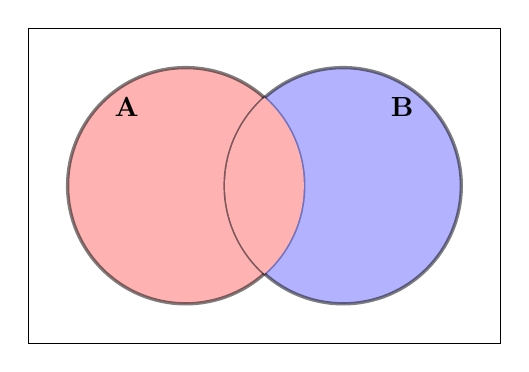
\begin{tikzpicture}
\def\circleA{(2,2) circle [radius = 1.5cm]} 
\def\circleB{(4,2) circle [radius = 1.5cm]} 
\draw (0,0) rectangle (6,4);

\onslide<3->{\draw[very thick, fill=red!60, opacity = 0.5] \circleA;
\node at (1.25,3) {\textbf{A}}; }

\onslide<4->{\draw[very thick, fill=blue!60, opacity = 0.5] \circleB;
\node at (4.75,3) {\textbf{B}}; }

\onslide<5->{
\begin{scope}[very thick]
\clip \circleA;
\fill[red!30] \circleB;
\end{scope} }

\end{tikzpicture} }
\end{center}
\end{frame}

\begin{frame}{Venn Diagram of Example 2b}
\begin{center}
\begin{tabular}{c|ccccc}
					&	\textbf{0--2} & \textbf{3--5} & \textbf{6--10} & \textbf{Over 10} & \textbf{Total} \\ \hline
\textbf{Foreign} 	& 37 & 21 & 12 & 30 & 100 \\
\textbf{Domestic} 	& 35 & 23 & 11 & 31 & 100 \\ \hline
\textbf{Total}   	& 72 & 44 & 23 & 61 & 200
\end{tabular}
\\[12pt]
\begin{venndiagram2sets}[labelA = \textbf{3--5}, labelB = \textbf{Dom}]
\onslide<2->{\node at (2.5,1.75) {23};}
\onslide<3->{\node at (1.5,1.75) {21};}
\onslide<4->{\node at (3.5,1.75) {77};}
\end{venndiagram2sets}
\end{center}
\onslide<5->{\[23 + 21 + 77 = 121\]}
\end{frame}

\begin{frame}{Example 3}
(a) If a single card is drawn from a standard deck, what is the probability of selecting a 3 or a club?	\newline\\
\onslide<2->{Number of 3s: 4} \newline
\onslide<3->{Number of clubs: 13}	\newline
\onslide<4->{Number of cards that are 3 and clubs: 1} 
\begin{align*}
\onslide<5->{P(3\text{ or club}) &= P(3) + P(\text{club}) - P(3\text{ and club})} \\[6pt]
\onslide<6->{&= \frac{4}{52} + \frac{13}{52} - \frac{1}{52}} \\[6pt]
\onslide<7->{&= \frac{16}{52}} \\[6pt]
\onslide<8->{&= \frac{4}{13}}
\end{align*}
\end{frame}

\begin{frame}{Example 3}
(b) What is the probability of drawing a face card or a red card?	\newline\\
\onslide<2->{Number of face cards: 12} \newline
\onslide<3->{Number of red cards: 26} \newline
\onslide<4->{Number of face cards that are also red: 6}
\begin{align*}
\onslide<5->{P(\text{face or red}) &= P(\text{face card}) + P(\text{red card}) - P(\text{face card and red})} \\[6pt]
\onslide<6->{&= \frac{12}{52} + \frac{26}{52} - \frac{6}{52}} \\[6pt]
\onslide<7->{&= \frac{32}{52}} \\[6pt]
\onslide<8->{&= \frac{8}{13}}
\end{align*}
\end{frame}
\section{Calculate the complement of an event}

\begin{frame}{Complements}
\begin{tcolorbox}[colframe=green!20!black, colback = green!30!white,title=\textbf{Complements}]
The \textbf{complement} of an event is the probability the event does \emph{not} happen.
\end{tcolorbox}
\vspace{10pt} \pause

Event: $P(A)$ \newline\\ 
Complement: $P(A')$
\begin{align*}
\onslide<3->{P(A) + P(A') &= 1} \\[8pt]
\onslide<4->{P(A') &= 1 - P(A)}
\end{align*}
\end{frame}


\section{Calculate "at least one" probabilities}


\begin{frame}{``At Least One" Probability}
\begin{center}
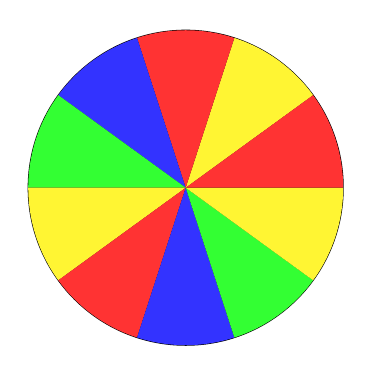
\begin{tikzpicture}
\draw (0,0) circle [radius = 2cm];
\foreach \x in {36,72,...,360}
\draw (0,0) -- (\x:2);
\onslide<2->{\fill[yellow!80] (0,0) -- (36:2) arc (36:72:2) -- cycle;}
\onslide<3->{\fill[red!80] (0,0) -- (72:2) arc (72:108:2) -- cycle;}
\onslide<4->{\fill[blue!80] (0,0) -- (108:2) arc (108:144:2) -- cycle;}
\onslide<5->{\fill[green!80] (0,0) -- (144:2) arc (144:180:2) -- cycle;
\fill[yellow!80] (0,0) -- (180:2) arc (180:216:2) -- cycle;
\fill[red!80] (0,0) -- (216:2) arc (216:252:2) -- cycle;
\fill[blue!80] (0,0) -- (252:2) arc (252:288:2) -- cycle;
\fill[green!80] (0,0) -- (288:2) arc (288:324:2) -- cycle;
\fill[yellow!80] (0,0) -- (324:2) arc (324:360:2) -- cycle;
\fill[red!80] (0,0) -- (2,0) arc (0:36:2) -- cycle;
}
\end{tikzpicture}
\newline\\
\onslide<2->{At least 1 is 1, \onslide<3->{or 2,} \onslide<4->{or 3,} \onslide<5->{$\dots$ or more.}}	\newline\\
\onslide<6->{The complement of \textit{at least one} is {\color{blue}\textbf{none}}.}
\end{center}
\end{frame}


\begin{frame}{Example 4}
Two dice are rolled. What is the probability of rolling a sum of at least 4?
\begin{center}
\begin{tabular}{c|cccccc}
			&	\textbf{1} & \textbf{2} & \textbf{3} & \textbf{4} & \textbf{5} & \textbf{6} \\ \hline
\textbf{1}	& 2 & 3 & 4 & 5 & 6 & 7 \\
\textbf{2}	& 3 & 4 & 5 & 6 & 7 & 8 \\
\textbf{3}	& 4 & 5 & 6 & 7 & 8 & 9 \\
\textbf{4}	& 5 & 6 & 7 & 8 & 9 & 10 \\
\textbf{5}	& 6 & 7 & 8 & 9 & 10 & 11 \\
\textbf{6}	& 7 & 8 & 9 & 10 & 11 & 12
\end{tabular}
\end{center}
\begin{align*}
\onslide<2->{P(\text{at least 4}) &= 1 - P({\text{less than } 4})} \\
\onslide<3->{&= 1 - P(2\text{ or } 3)} \\
\onslide<4->{&= 1 - \frac{3}{36}}
\onslide<5->{= \frac{33}{36}} \onslide<6->{ = \frac{11}{12}}
\end{align*}
\end{frame}

\begin{frame}{Example 5}
A certain blood test can determine the presence of a bloodborne pathogen 97\% of the time (that is, if 100 people have the pathogen, the test will confirm true for 97 of them). If 4 people with the pathogen are given the test, find the probability that the test is accurate for at least one of them.	
\begin{align*}
\onslide<2->{P(\text{at least 1 accurate}) &= 1 - P(\text{none are accurate})} \\
\onslide<3->{&= 1 - P(\text{1st inaccurate})\times P(\text{2nd inaccurate}) \cdots} \\
\onslide<4->{&= 1 - (0.03)^4} \\
\onslide<5->{&= 0.99999919}
\end{align*}
\end{frame}


\section{Calculate the odds of an event}

% Addition Rule
% General Addition Rule
% Complement Rule
% At least n
% Odds

\end{document}